\section{Crowd-Shared Wireless Mesh Network Management}
\label{sec:architecture}

The underlying problem with PAWS or any crowd-shared network is that they serve as single point of Internet access to guest users within the coverage of the wireless router and hence, they have no provision to extend the coverage when no bandwidth is being shared. Based on our experience from the trial PAWS deployment, PAWS routers were always not available for certain periods, because sharers needed all the bandwidth of their broadband connection or due to other reasons, such as economic constraints placed on home users in underprivileged areas where they are forced to conserve energy by turning off the routers at nights. In this respect, Fig. \ref{fig:paws-avail} presents a six-month view of the PAWS routers status (available/unavailable) logs demonstrating that not a single router was available continuously over the entire duration. These observed user behaviors entail significant challenges for the successful adoption of PAWS. 

\begin{figure}[t]
\begin{center}
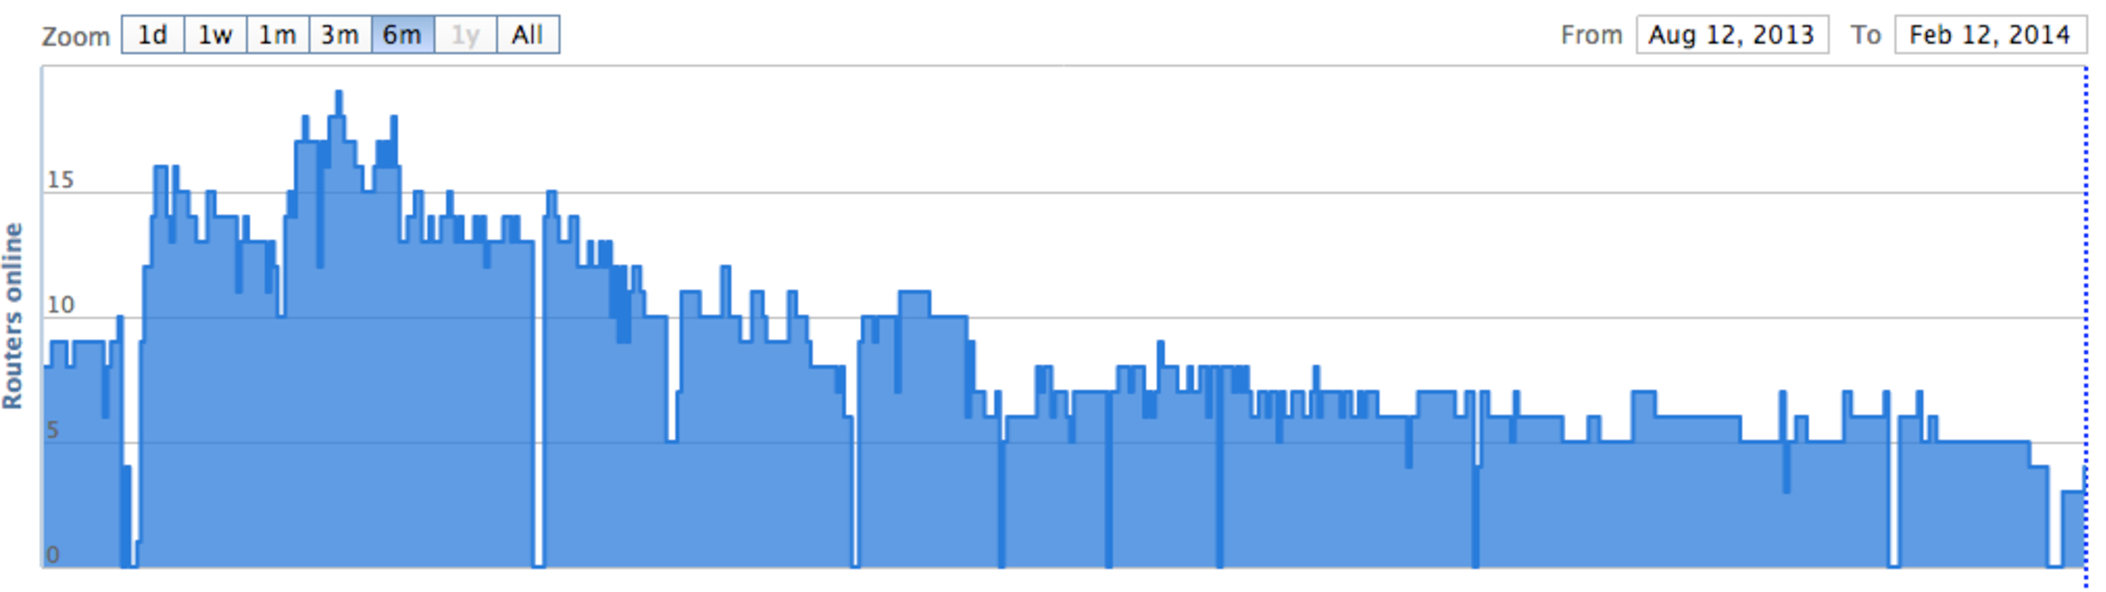
\includegraphics[width=1\linewidth]{paws-avail.pdf}  
\caption{PAWS routers availability.}
\label{fig:paws-avail}
\end{center}
\end{figure}

A potential solution to this problem is to extend the PAWS network as a crowd-shared mesh network. Such a network would allow home network users to share part of their own broadband connection to the public for free while also connected to each other as a wireless mesh providing extended coverage. Extending PAWS to a crowd-shared mesh network departs from the norm: multiple users from different ISPs form part of the mesh network to provide free Internet connectivity, while most wireless community mesh networks today are operated by a single organization. This raises important questions regarding the operation, configuration, and management of crowd-shared mesh networks.  

In \cite{LCDNet}, we describe a holistic approach of coupling both social and economic incentives in designing future networks allowing the extension of the stakeholder value chain to include more than the two traditional parties (consumer and internet service provider). Such an approach would provide opportunities for non-governmental organizations and local governments (driven by social goals rather than economic) to become virtual network operators. Enabling a third party to federate such wireless home networks would reduce the operating expenditures for network operators as well as enable new economic models for revenue creation from currently underutilized infrastructures.

To this end, in \cite{EWSDN} we presented an evolutionary architecture that enables third-party stakeholders, such as local government or other non-governmental organizations, to become virtual network operators, reducing the costs of network operators to setup and manage new infrastructures to extend access to their Internet backhaul. With the advent of SDN, there are more opportunities for network operators to deploy and manage in large scale such as open public wireless networks. In \cite{EWSDN}, we use SDN to create the notion of Virtual Public Networks (VPuN), i.e., crowd-shared home networks created, deployed and managed through an evolutionary SDN control abstraction. This offers more flexibility to users and multiple network operators, allowing them to share and control the network, while providing opportunities for new stakeholders to emerge as virtual network operators. Although originally intended for crowd-shared wireless networks such as PAWS, we believe the VPuN architecture could also solve the above mentioned challenges imposed by crowd-shared wireless mesh networks. Although a mesh network allows resource pooling across multiple paths and robustness to failures, it entails significant challenges in terms of configuration and management. In particular, a crowd-shared mesh network for PAWS spans home networks interconnected as a mesh across multiple ISPs, all of which may be operated independently. Instead of fostering the collaboration among multiple operators, which has not been very successful in the past, we consider outsourcing the mesh network operation and management to a third party VNO leveraging on SDN.

